\documentclass[11pt]{article}
\usepackage[sorting=none]{biblatex}
\usepackage{graphicx} 
\usepackage[font=scriptsize,labelfont=bf]{caption}
\usepackage[a4paper, total={5.5in, 8.5in}]{geometry}
\usepackage{cleveref}
\usepackage{wrapfig}
\usepackage{subcaption}

\addbibresource{bibliography.bib}

\title{Xcorr Reimplementation Bachelorthesis}
\author{Michael zusmanovskiy}
\date{November 2024}

\begin{document}

\begin{titlepage}
    \begin{center}
        \LARGE
        Applied Computer Science

        \vspace{1cm}
        
        \LARGE
        Bachelorthesis

        \vspace{1cm}
            
        \LARGE
        \textbf{Re-implementation of the X-Corr algorithm in Python and improvement of scoring using predicted spectra}
            
        \vspace{1cm}

        \LARGE
        \textbf{Author}
        
        Michael Zusmanovskiy, 108019231182
        
        \vspace{1cm}
        
        \LARGE
        \textbf{Supervisors}
        
        Jun.-Prof. Julian Uszkoreit
        
        M.Sc. Dirk Winkelhardt
            
        \vfill
        
        \begin{figure}[ht]
            \centering
            \includegraphics[width=0.2\textwidth]{figs/Ruhr-Universität_Bochum_logo.svg.png}
        \end{figure}
            
        \Large
        Ruhr-Universität Bochum\\
        
        Submission date: 30. 12. 2024
            
    \end{center}
\end{titlepage}

\tableofcontents
\newpage

\section{Introduction}
\subsection{Fundamentals}
Mass Spectrometry (MS) is a method for measuring the mass to charge ratios (m/z) of components in a  chemical substance sample and analysis of its molecules \cite{mass-specrometer}. MS has a variety of applications \cite{ms-applications} reaching from forensic analysis, where it is used to trace evidence , over environmental analysis, for example to keep track of pollution or test drinking water, to clinical purposes where MS is used for genomics research or diabetes research \cite{ms-diabetes}.
Before mass spectrometry can be performed, the sample has to be prepared meaning that it is turned into a state that is a valid input for the mass spectrometer. This is done by either converting it into a gas phase for Gas Chromatography or into a liquid phase for Liquid Chromatography. In Gas chromatography the molecular components are separated by vaporization and dilution of the sample on basis of attributes like weight, size, or boiling point. Liquid chromatography on the contrary separates components on basis of how fast they travel trough a liquid phase, this can be for example because of the difference of the polarity of the liquid phase and the components of the sample. Of course, the exact workflow is dependant on the Instrument that is used. Mass spectrometers exist in various variants e.G. MALDI-TOF MS, Triple Quadrupole MS, Hybrid Linear Ion Trap Orbitrap MS etc.  \cite{mass-specrometer-types} however regardless of their type they usually follow the same steps \cite{mass-specrometer, what-is-mass-spectrometry}: 

\begin{enumerate}
\item After the sample preparation, the sample is ionized, meaning that ions are generated. A common approach in gas chromatography is electron bombardement where the molecules are passed through a ionization chamber with accelerated electrons. The electrons collide with the molecules, break their bonds and turn them into fragments. A different approach in liquid
chromatography is electrospray chromatography where the liquidified sample is sprayed into an electric field where it evaporates.
\item The produced ions are sorted by their mass-to-charge ratios by a mass analyser. How this is done is dependant on the machine that is used.
\item After the sorting of the ions a detection system determines the relative abundances for each observed mass-to-charge (m/z) value.
\end{enumerate} 

The output is a mass spectrum which is a plot that yields the m/z values on the x-axis and the abundances on the y-axis. The m/z value is the mass of a particle divided by its electrical charge. The abundances are normalised to the highest abundance peak in the spectrum, meaning that the highest peak is 1 and all other peaks have a value relative to it [\cref{fig:peptide-example}]. 

Tandem mass spectrometry (MS/MS or \(MS^2\)) can be understood as an extension of mass spectrometry. It is used for the analysis of peptides and involves multiple stages, where in the first stage the entire sample is analysed with a mass spectrometer, then one ion is selected for further analysis and on the next stage only this isolated ion is analysed by another MS run \cite{tandem-mass-spectrometry}. This is realized by connecting two analyzers behind each other in "tandem", which are connected by a collision cell. In the first MS run ions are analyzed, those are the so called "precursor ions" and some of then are selected by their m/z value. The selected precursor ions are then even further fragmented into smaller peptide chains by an inert gas, after which they are let into the second spectrometer \cite{tandem-mass-spec-deutsch, tandem-mass-spec-yt}.

Since every peptide sequence produces its own unique mass spectrum, it can be used as its unique fingerprint to identify it in a sample.
\begin{figure}[ht]
\centering
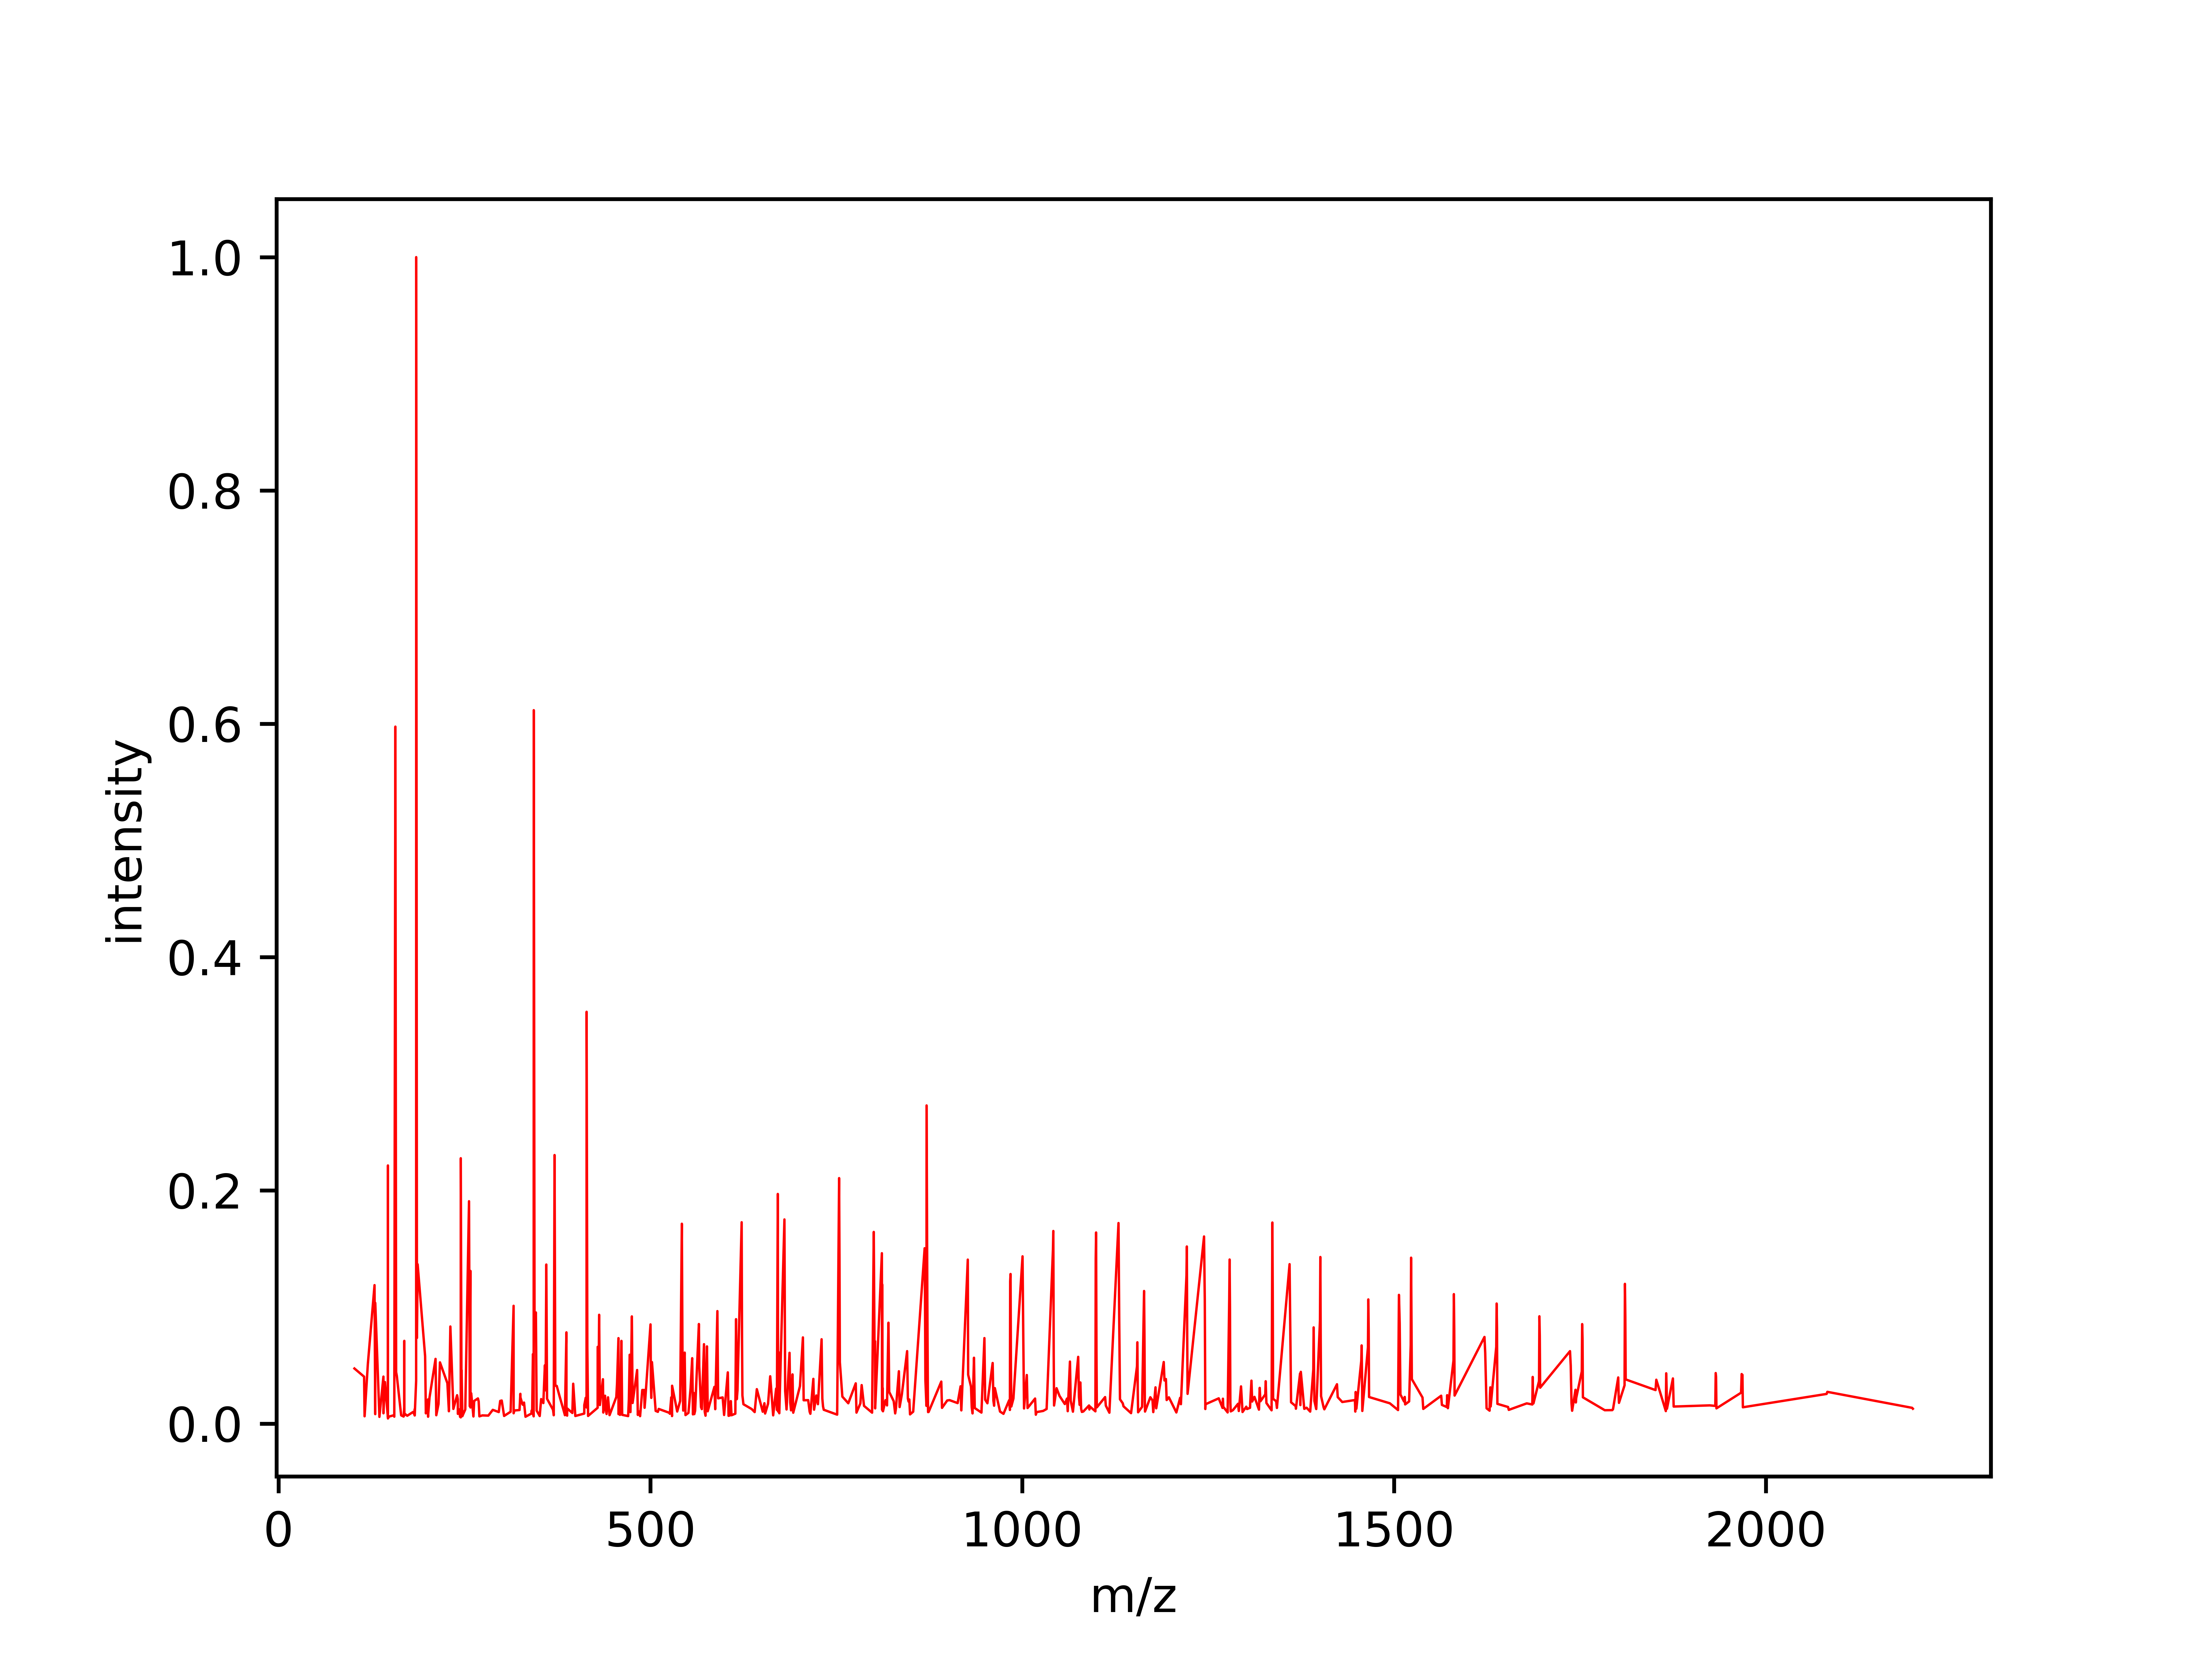
\includegraphics[width=0.8\textwidth]{figs/peptide.png}
\caption{MS spectrum of the peptide "LAADEDDDDDDEEDDDEDDDDDDFDDEEAEEKAPVK" retireved from the human genome}
\label{fig:peptide-example}
\end{figure}
\begin{figure}[ht]
\centering
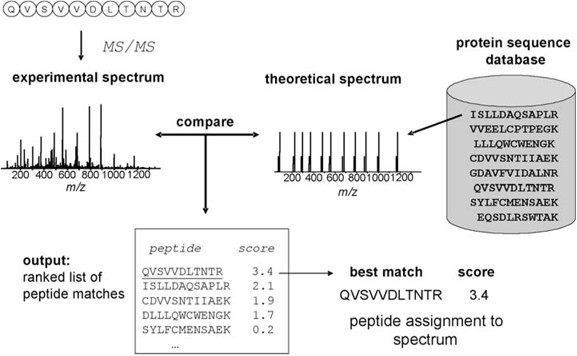
\includegraphics[width=0.8\textwidth]{figs/database_search.jpg}
\caption{Peptide identification with the database searching approach \cite{Nesvizhskii2007}}
\label{fig:database-search}
\end{figure}
Tandem MS searching is used for peptide identification within a mass spectrometry scan. Proteomics software that deals with the problem of identifying protein/peptide identification can fall into the category of database searching, where the search is performed against a database, and de novo searching, where peptides are deduced without a database. The de novo approach is typically less accurate than the database method, while the database method works only if the selected database with which the search is done indeed contains the searched proteins/peptides.

This thesis is revolving around the database searching approach. The general concept of tandem MS database searching is described in \cref{fig:database-search}. An experimental spectrum from an MS/MS run generated by an unknown peptide sequence has a certain mass,  if peptides retrieved from a protein database have a mass close to the experimental peptide, the MS/MS spectrum is compared to their "theoretical spectra". To understand how a theoretical spectrum is generated, it is first necessary to understand the concept of ion fragmentation. 

In a mass spectrometer peptide bonds can be broken in different positions of the peptide, from the N-terminal the a,b,c positions, and from the C-terminal the x,y,z positions. Usually the b and y positions are selected for fragmentation. In an MS/MS scan each abundant peak that is noticably larger than the noise peaks, optimally is produced by one fragment ion. When annotating a spectrum from the C and N terminal end, the m/z distances are calculated between the most abundant peaks, this can give an insight about one amino acid, and finally the entire peptide sequence \cite{b-y-ions}.

A theoretical spectrum of a peptide from a database is created by the b and y series, for this the sums of the first, then first and second, then first, seconds and third etc. amino acids are calculated, until the end of the peptide sequence, for both the b and y ions, considering charges.

\subsection{Motivation}
\subsubsection{Comet Xcorr in detail}
Comet is an open source proteomics Tandem MS/\(MS^2\) database search algorithm/tool written in C++ for searching spectrum data against sequence databases and identification of peptides, that in 2012 emerged from the SEQUEST database search tool from the University of Washington that was written in 1994 \cite{comet-search-tool}. It supports multithreading and is highly parametrizable. For the peptide identification the tool computes multiple scores that evaluate how close a sample peptide is to a peptide from a genome database that it is compared to. One of these scores is the "Xcorr", which will be the focus of this thesis. 

To calculate the Xcorr value and other scores the algorithm first performs a filtering of peptides from a given database. If a sample spectrum has a precursor ion mass of e.g 1500 dalton, the algorithm considers only those peptides from the database that have a mass close to it, e.g with a tolerance of  $\pm$0.005 dalton, meaning that a peptide with a mass of e.g. 1500.001 would be selected for further analysis. All database peptides outside of this mass boundary are discarded.

For these filtered peptides it is assumed that one of them could possibly have generated the sample mass spectrum. The program constructs a spectrum from the peptides by generating all possible m/z values from the 'b' and 'y' series of the peptide, which in the following will be referred to as the "theoretical spectrum" \cite{comet-first-paper}. 

In the next step comet computes how similar the sample mass spectrum is to the obtained theoretical spectrum. In science many methods for the computation of similarity between signals are used, e.g euklidean distance or frequency domain analysis, comet uses the cross correlation approach. Before the cross correlation can be computed, comet preprocesses the sample and theoretical spectrum by "binning". Comet has the option to perform binning with low resolution i.e. a bin size of 1.0005, or high resolution with a bin size of 0.02. 

Since in 1994 it was not entirely possible to predict the intensities of 'b' and 'y' ions, the theoretical spectrum is assigned intensities of 50 on the b and y ion generated m/z positions \cite{deeper-look-into-comet}. For the sake of slightly increasing tolerance and making the theoretical spectrum peaks into a "bell shape", neighboring m/z values, meaning $\pm$1 m/z, receive an intensity of 25. 

After the binning stage, the binned experimental sample spectrum is further processed, how exactly this processing works was found out by personal communication by email with the comet developer Jimmy K. Eng.. The binned experimental spectrum is divided in 10 equal windows, inside of each of these windows, all values are normalised between 0 and 50, meaning that the highest peak recieves an intensity of 50, and all other peaks in the bin recieve a value relative to it. This is done for the purpose of making the experimental spectrum look similar to the theoretical spectra, and enhance possibly relevant peaks.

For the Xcorr, the similarity at zero offset is first determined, after that the binned arrays are shifted by $\pm$75 dalton and the correlation is determined at each offset. The background similarity is defined by computing the mean of all correlation values without the one at zero offset. The xcorr is then similarity at 0 offset minus background similarity \cite{xcorr-function}.

\subsubsection{Peptide intensity prediction}
Peptide prediction algorithms are able to predict \(MS^2\) peaks from given peptide sequences with the help of various machine learning models trained on large amounts of \(MS^2\) data. MS2PIP\cite{ms2pip} (short for \(MS^2\) peak instensity prediction) is a command line peptide intensity prediction tool which also exposes a Python API.

\subsubsection{Goals}
The goal of this work is to combine the comet cross-correlation scoring algorithm
with the peptide intensity prediction of MS2PIP to reveal whether replacing the Comet generated theoretical spectrum with the predicted spectrum of MS2PIP will yield better results in peptide identification, and with this, to find a new and possibly even more accurate method of peptide identification.

As comet is written in the C/C++ Programming Languages and MS2PIP is a Python Api, it is first of all necessary to translate the Comet cross-correlation scoring algorithm to the python programming language as accurately as possible. Next, the theoretical spectrum containing only m/z values without any abundances created by comet will be replaced by the predicted spectrum of MS2PIP. Performance regarding computational speed and identified peptides will be then compared to the initial comet algorithm, and the to python translated comet.

\subsubsection{Reference comet run}
To later compare the identified peptides and the performance of the original comet implementation and this implementation, a reference run with the original Comet search tool was performed. The number of used processing threads was set to 10, the peptide mass tolerance was set to 20 parts per million (ppm), the amount of missed cleavages was set to 2, the valid ms level is set to two. The run was done with high resolution binning, that means a bin width of 0.02 was used. The variable modification oxidation of the amino acid methionine (M) and static modification carbamidomethylation of cysteine (C) were considered.

\section{Implementation of the Xcorr algorithm in Python}
\subsection{Reading in Spectrum data}

As aleready mentioned in the Goals section, Python is selected as the Programming language for this work. Before implementation, it is first necessary to have human genome data to work with, for this purpose, LFQ Orbitrap data was used as the sample, specifically in the mzml format which is a xml based format for storing mass spec scan data. Each scan has a unique scan id and contains binary coded information about the scan start time, MS level, base peak m/z and intensity, lowest and highest observed m/z, the m/z array and the intensity array e.t.c.. In case of a \(MS^2\) scan, it additionally contains information about the selected precursor ion(s) like e.g. its charge state.

The search is done against data of the Homo sapiens (Human) genome in the fasta format which stores protein primary structure and serves as the "database". Each protein entry inside the file has a header with a unique name, id and description. The used fasta file was obtained from the uniprot Knowledgebase and has the id UP000005640.

Acessing these files with Python was done with the help of the pyteomics python framework \cite{pyteomics, pyteomics-five-years} which contains many tools for analysis of proteomics data. 

\subsection{Creating a peptide index list}
For efficient identification of peptides it is first necessary to create a compact list that contains all masses, and peptides that have this mass, from the fasta database file. In the following this list will be referred to as the "peptide index". While iterating through the fasta database, the retrieved sequences are \textit{in silico} digested, meaning that the function of the human digestive system is simulated. In the human body peptides that are too large for the small intestine are cleaved by the enzyme trypsin, and are called "tryptic peptides". This digestion is realized by cutting the sequences after the amino acids Arginie (R) and Lysine (K), except for those sites where R or K are followed by Proline (P). The general regular expression for this is "(?$<$=[KR])(?!P)". For this matter, the pyteomics library function parser.cleave was used, for each peptide that was cleaved off, the resulting peptide length is restricted between 6 and 50 amino acids, and a maximum of 2 missed cleavages is allowed, meaning that at most two spots that are matched by the regular expression are "overlooked". 

The resulting peptides are all in a unmodified state, so for the program to recognize possible modified peptides in a scan from the mzml file, it is necessary that for every peptide that has been cleaved from a sequence from the fasta database file, all its isoforms are generated. Those peptides that contain an "X", i.e. an unidentified amino acid, are ignored. The generating of isoforms is achieved by the pyteomics library function isoforms from the parser module, which takes in one peptide cleaved from the database at a time, applies fixed modifications i.e. modifications that are always applied, and variable modfications, for which all possible combinations are generated. Examplary like in the reference comet run, the static modifications Carbamidomethylation of Cysteine (C) as well as the variable modification Oxidation of Methionine (M) have been taken into account. The amount of maximum modifications is set to three, meaning that in one peptide at most three amino acids can be affected by a variable modification.

For every generated isoform, the mass is calculated. This mass is added to a dictionary as the key if it does not exist yet, and the according peptide as the value. Since multiple peptides can have the same mass, it is possible that for a mass/key value are multiple peptides stored. Next, the dictionary is converted to list which is sorted by the mass in ascending order [\cref{fig:peptindex}]. The reason for this is that a python dictionary is unordered and "unindexable", and since binary search will be performed in the following on the peptide index, this is an issue.
 
\subsection{Multiprocessing}
After generating the peptide index list, a pool of user specified amount of processes is created in order to increase performance and use as many computer resources as possible. A manager from the python multiprocessing library is used to share the previously generated peptide index between the pool processes. 

The program starts iterating over the spectra inside the mzml sample file, and does so until all spectra are read. It loads user defined amount of spectra into a buffer, which is accessed by the process pool. A process loads one spectrum scan from the buffer and proceeds with the identification, meaning that the peptide index is searched for a possible close match for the spectrum.

\subsection{Filtering of candidate peptides}
Each single process calls the identification function, which does the following:
It iterates over the tree structure of the mzml file, and it is first checked whether the MS level is 2. If this is the case, the program iterates over all possible precursors and selected ions, where it first calculates the mass in dalton of the selected ion from the retrieved mass to charge value. 

The program proceeds with a rough filtering of peptides that can come into question for the given scan. This is done by a lookup into the peptide index where it is searched for peptides that have a mass close to the mass of the selected precursor ion. The tolerance for a canditate peptide is 20 parts per million (ppm), that means between a mass of $\pm$ (spectrum mass * 0.00002).

The lower and upper tolerance bounds are first calculated. The peptide index is a list meaning that it is indexable, and the masses are sorted in ascending order, that means that it is possible to efficiently get the upper and lower indices of the peptide index entries by performing binary searching on the list. A binary search function is searching for the lower index of the peptide list first, and returns the first index of the list where the mass is $\ge$ the calculated lower bound. The upper index is searched the same way. After getting the upper and lower indices, the process gets a slice from the peptide index including all peptides that are possible candidates for scoring. E.g if the lower bound for the mass is 1033.6777 and the upper bound is 2190.5454, the slice would be between the second line and the second last line in \cref{fig:peptindex}.
\begin{wrapfigure}{r}{0.5\textwidth}
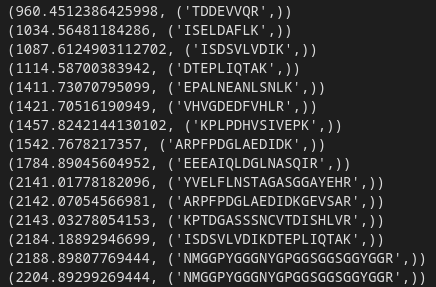
\includegraphics[width=\linewidth]{figs/peptindex.png} 
\caption{Peptide index list generated from the fasta database file}
\label{fig:peptindex}
\end{wrapfigure}

\subsection{Binning}
The mass-to-charge values and its corresponding intensities are retrieved as two separate numpy arrays from the mzml file and are sorted in a way that the m/z values are in ascending order, and every m/z value in the m/z array has its intensity stored in the intensity array on the exact same index.

The process continues with what in the original comet implementation is referred to as "binning". First, the values in the intensity array are normalised between 0 and 50. Depending on the bin size, the bin index of a m/z value is calculated by dividing the m/z by the bin width. A numpy bin array is created, its size depending on the biggest m/z value in the m/z array, and since an m/z array from the mzml file can have values up to 2000, the bin array can have a size of 100.000. The bin array is filled with the intensites from the intensity array on the calculated index. In case there are 2 intensities on the same index, like in the comet implemenation, only the highest intensity is stored. Like in comet, the binned experimental array is processed by dividing it into 10 equal sections and normalisation is performed within them.
\begin{wrapfigure}{r}{0.5\textwidth}
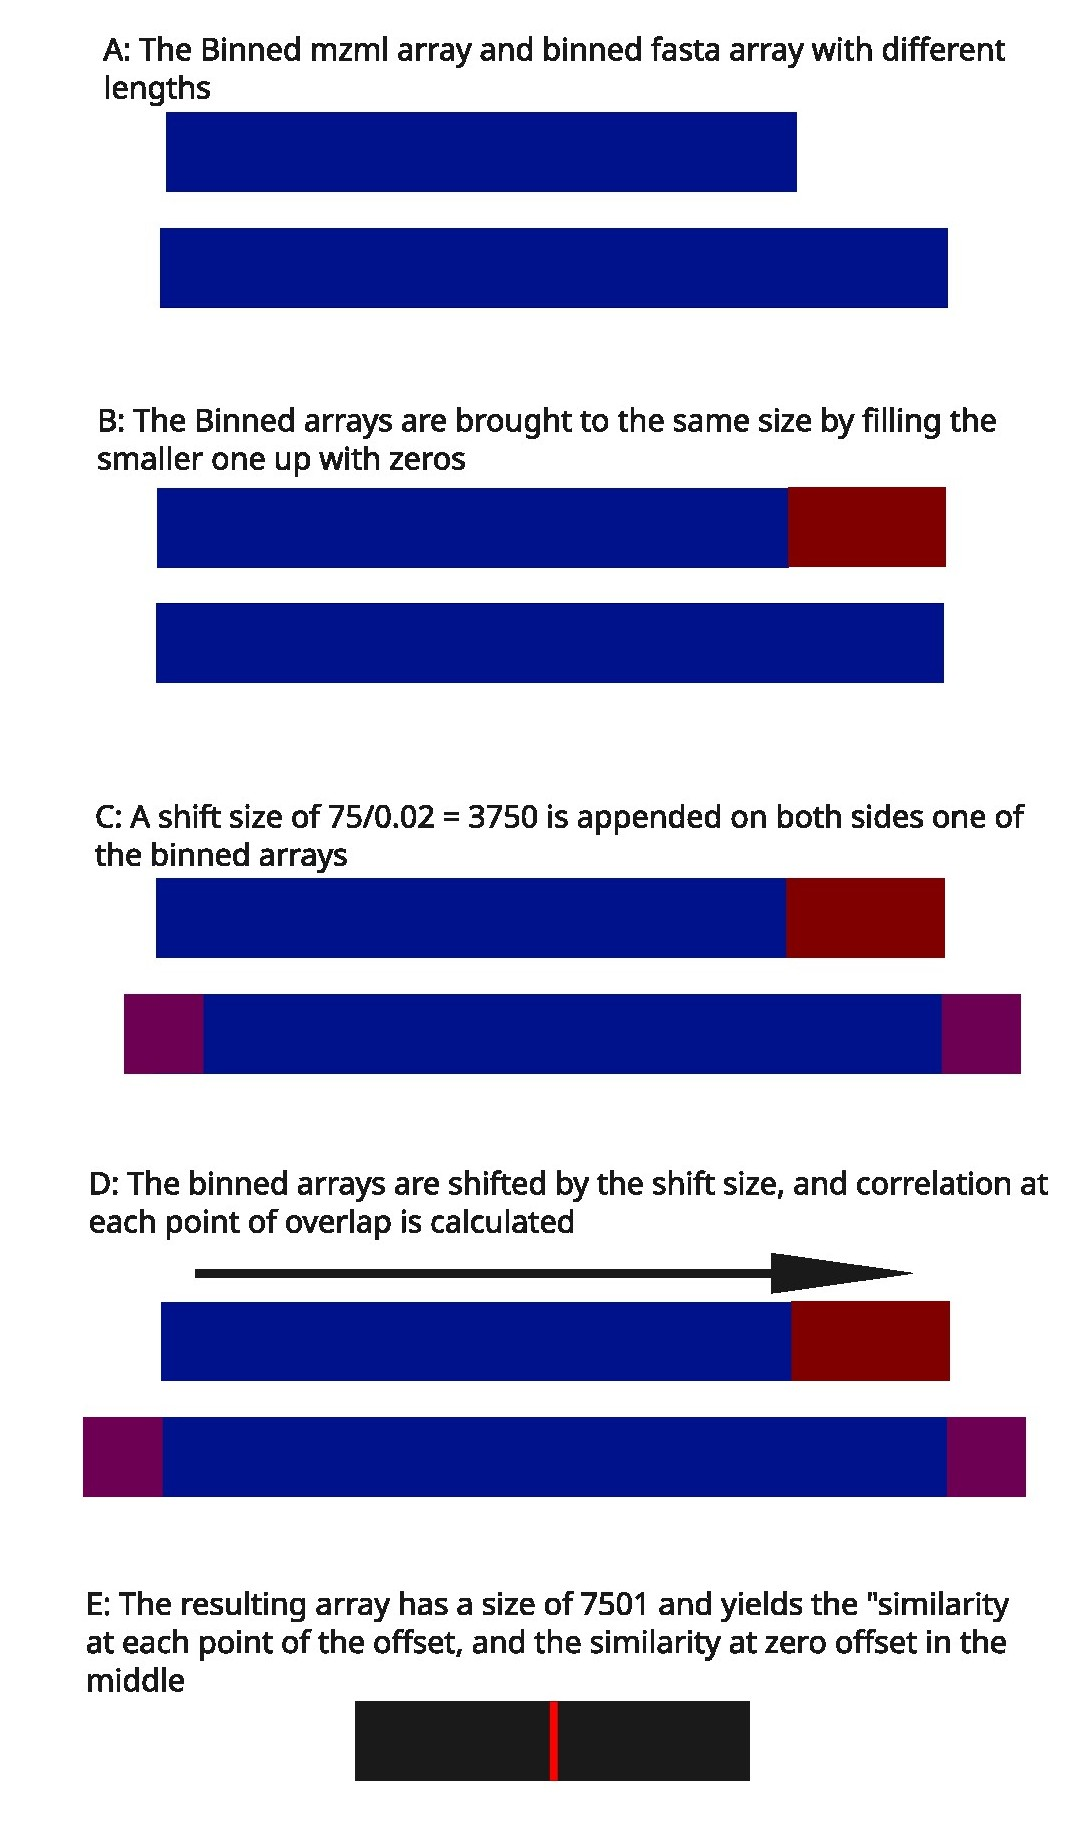
\includegraphics[width=\linewidth]{figs/crosscorr.jpg} 
\caption{Preprocessing the binned arrays before correlation}
\label{fig:corr}
\end{wrapfigure}
The program now proceeds with generating fragment m/z values of the peptides from the previously retrieved array slice with candidate peptides. This is done by a seperate function for every peptide in the slice which takes in the peptide as a string and the maximum charge of the selected precursor ion - 1 as the parameters. Like in the initial reference comet run, the maxcharge is limited to 3. The fragmentation function returns a list with m/z values, which is the "theoretical spectrum" of the candidate peptide, and binned the same way as the spectrum retrieved from the sample mzml file, except that this fragmentation m/z list has no corresponding list containing intensities. In this case the bin array index is calculated the same way, but on the index position the bin array is filled with a 50, and neighboring bins are filled with a value of 25. 

\subsection{Peak intensity prediction with MS2PIP}
In case the user of the tool decides to run the program with predicted spectra instead of the theoretical spectra, the program runs the predict\_spectrum function on the peptides. The Pyteomics library and the MS2PIP library have different ways of labeling/marking modifications of a peptide, so the peptide retrieved from the peptide index has to be parsed by a Pyteomics parser which takes in a Pyteomics formatted peptide string and returns the peptide as a list of labels, this list is then iterated over and a MS2PIP style-formatted modification string is generated. The plain isoform of the peptide and its modification string are then fed into the MS2PIP predict function, which returns an array of predicted m/z values and its corresponding predicted intensity array.


\subsection{Xcorr scoring}
After the sample spectrum and the theoretical spectrum have been binned, they have to be brought to the same length. This is achieved by filling up the binned theoretical spectrum with zeros in case it is smaller than the binned sample spectrum. If the binned sample array is smaller, it is simply cut to the right length. 

The correlation is calculated by the correlate function from the numpy library with the mode "valid". In the comet implementation the binned sample and binned theoretical spectrum are shifted by $\pm$75 dalton, which corresponds to a shift of 75/0.02 bins, where at each overlap the dot product is calculated. The resulting array has a size of 3750 + 3750 + 1 = 7501, a shift of 3750 bins in each direction and the dot product at zero offset. The correlation at zero offset corresponds to the entry at index 3750 in the resulting array, which is exactly the middle entry. To calculate the background similarity, the entry at the middle index is removed and the mean over all remaining entries in the correlation array is calculated. The Xcorr score is computed by subtracting the background similarity from the similarity at zero offset, then divided by 10.000.[\cref{fig:corr}].

\subsection{Output}
The process returns and adds all identified results for a peptide from the sample mzml file to a result list. When the buffer is fully consumed, all results are printed to a tsv file in tab separated format. One result consists of the scan number which is unique for every entry inside of the sample mzml file, the charge of the precuror ion, the mass of the experimental neutral precursor ion from the mzml file, the calculated neutral mass of the theoretical peptide that has been selected for matching, the Xcorr score, the amount of matched ions, meaning the amount of sites where on zero shift there are non-zero values in both binned arrays, the amount of total ions of the theoretical spectrum and the plain unmodified peptide.


\subsection{CLI}
To make usage comfortable, a CLI is implemented. This was done with the help of the Typer Python library. The general usage is defined as "cli.py [OPTIONS] SAMPLE\_FILENAME PROTEIN\_DATABASE" in the terminal, where "SAMPLE\_FILENAME" is a required argument and placeholder for the sample filename in the mzml format as a string, and "PROTEIN\_DATABASE" the string for the database filename of the human genome respectively, in the fasta format. 

The CLI provides additionally three options: The "--p" flag followed by an integer sets the amount of processes to use for multiprocessed identification. If this flag is not set, the program works with a default value of cpu\_count()-2, where cpu\_count() returns the amount of processes the used machine can provide. The "--s" flag followed by an integer specifies the amount of spectra that the processes load and buffers at a time. The default amount is 5000. If the "--ps" flag is set, the program will work with the predicted spectra instead of the theoretical ones.

The user can get a help-text by typing "cli.py --help" in the terminal, which contains the above mentioned information.

\section{Results}
To compare the execution times and identification of comet and this implementation, a small fasta database file was created, which contains the top 110 peptides that matched in the initial previously described comet run. Both versions of the Python program were run with the exact same parameters with 4 processes with a ssh remote connection on a data center.
An examplary output of the Python program is shown in \cref{fig:output}, sorted in descending order by xcorr scores.
\begin{figure}[ht]
\centering
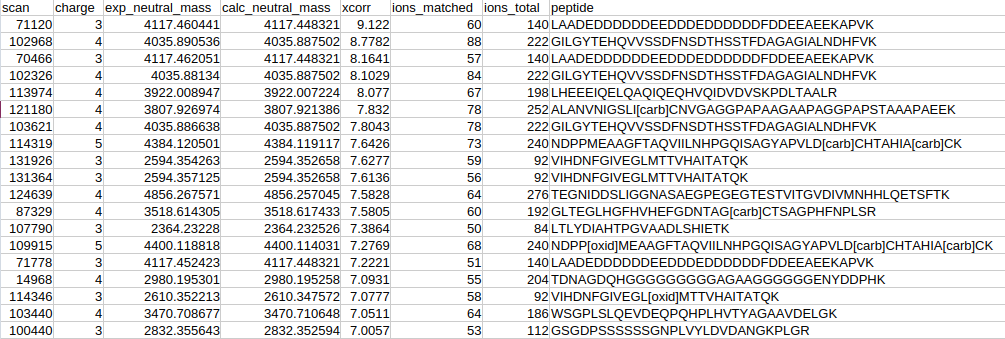
\includegraphics[width=1\textwidth]{figs/output.png}
\caption{An example output of the program, used theoretical spectra for identification}
\label{fig:output}
\end{figure}

\subsection{Identification comparison}
Although the resulting xcorr scores are not exactly matching with the scores of the original comet implentation, this implementation manages to compute scores that are close to the ones in comet. This is demonstrated in \cref{fig:scatterplot}. The x-axis represents the scores produced by the python program, the y-axis the scores of comet. For this plot only the highest score was selected for every scan number. The scatterplot dots align mostly in a straight line, which demonstrates that the scores of the python Program are close to the scores of comet. The scatterplot also contains outliers which shows that some scores are not matching, the reason for the not exact matching is that comet has additional steps in preprocessing the binned spectra, and comet also uses a fast scoring algorithm which was not taken into account in this python implementation. 
\begin{figure}[ht]
\centering
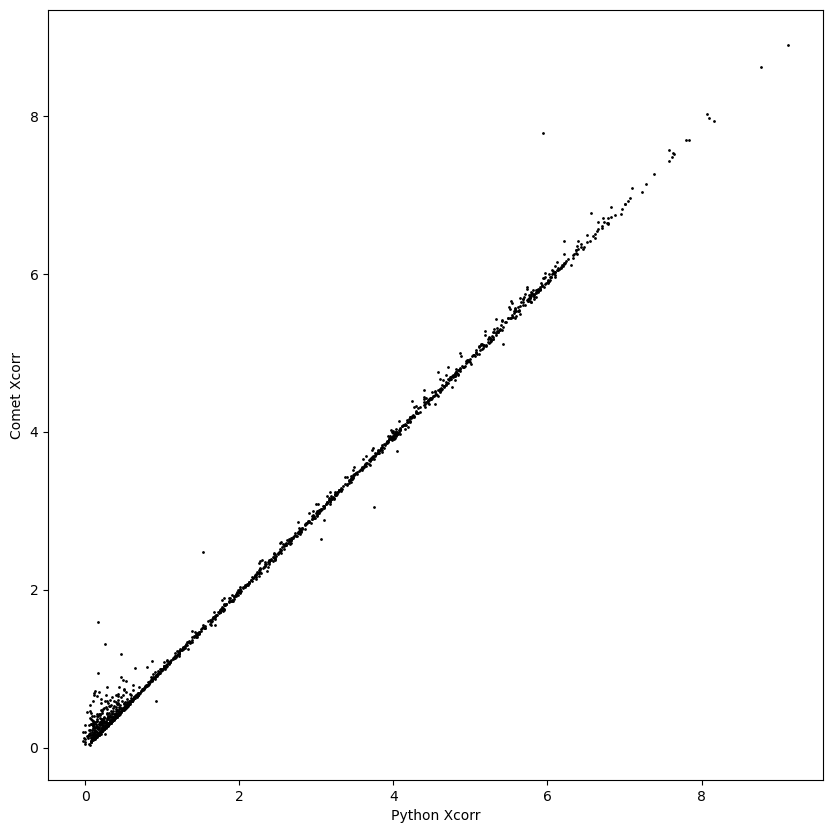
\includegraphics[width=0.8\textwidth]{figs/scatterplot.png}
\caption{Scatterplot between the comet xcorrs and in python replicated xcorrs. For each scan number in the results only the highest xcorr value was selected.}
\label{fig:scatterplot}
\end{figure}

Now that the scores generated by the Python program using theoretical spectra are close to the scores in Comet, a comparison between scores using predicted spectra with Ms2pip can be done. The scores of the Python program with the theoretical spectra have been plotted against the scores using predicted spectra in \cref{fig:scatterplot_predicted_theoretical}. As expected, the correlation between both scoring is low.

\begin{figure}[ht]
\centering
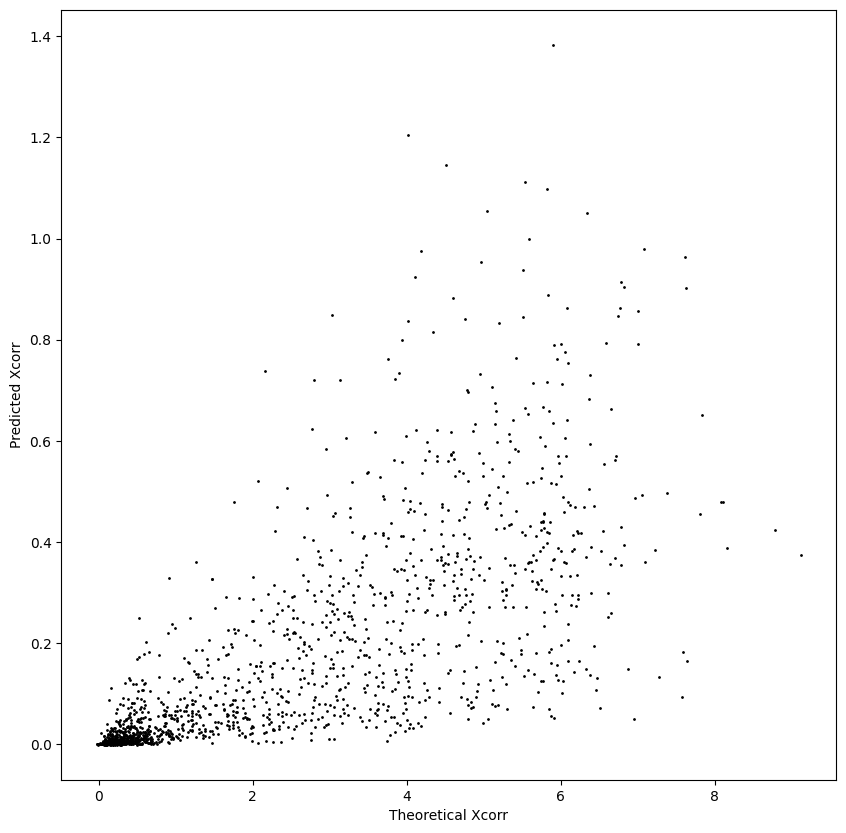
\includegraphics[width=0.8\textwidth]{figs/scatterplot_predicted_theoretical.png}
\caption{Scatterplot between the scores using theoretical spectra and predicted spectra in python. For each scan number in the results only the highest xcorr value was selected.}
\label{fig:scatterplot_predicted_theoretical}
\end{figure}
An example for a good match is shown in \cref{predandtheo}. The blue peaks are generated by the processed experimental spectrum from the scan 71120, and the red peaks are the theoretical spectrum for the peptide "LAADEDDDDDDEEDDDEDDDDFDDEEAEEKAPVK". As can be seen, most of the red theoretical spectrum peaks in \cref{predandtheo}(a) match the highest blue peaks. In this case, 60 of the total 140 theoretical spectrum ion peaks match a blue peak. 

For the predicted spectrum matching in \cref{predandtheo}(b) for the same scan, 70 red peaks were predicted in total by MS2PIP, 25 of which are matching the peaks of the blue experimental spectrum.

\cref{predandtheocorr} demonstrates that the highest correlation was calculated at zero offset of both the experimental and theoretical/predicted spectra. There are notably fewer background similarity peaks in the correlation array of the predicted spectrum, demonstrating that the predicted spectrum is more accurate than the theoretical one.

All of this are high indicators that the experimental spectrum with scan number 71120 might indeed be produced by the peptide "LAADEDDDDDDEEDDDEDDDDFDDEEAEEKAPVK".

Despite the predicted spectrum closely matching the experimental spectrum in \cref{fig:predict}, the score is much lower then the score for the theoretical spectrum match. This score is also not high in comparison to other scores using predicted spectra, which go up to 13.8. This is caused by the normalisation of the entire spectrum to the highest peak, in \cref{fig:predict} exist three peaks that are significantly more abundant than the rest of the peaks, which are small in comparison. The products between most of the binned array entries are low, which leads to a low Xcorr score. This is also apparent in \cref{fig:scatterplot_predicted_theoretical}, which shows that there is almost no correlation between the scores for the predicted and theoretical matching.

To address this problem, the same approach as in comet is used. Instead of normalising both predicted and experimental spectra to the highest peak over the entire m/z interval, both of the spectra are divided into ten equally long windows, and on each of these windows normalisation is performed.

\begin{figure}
\centering
\begin{subfigure}[b]{1\textwidth}
    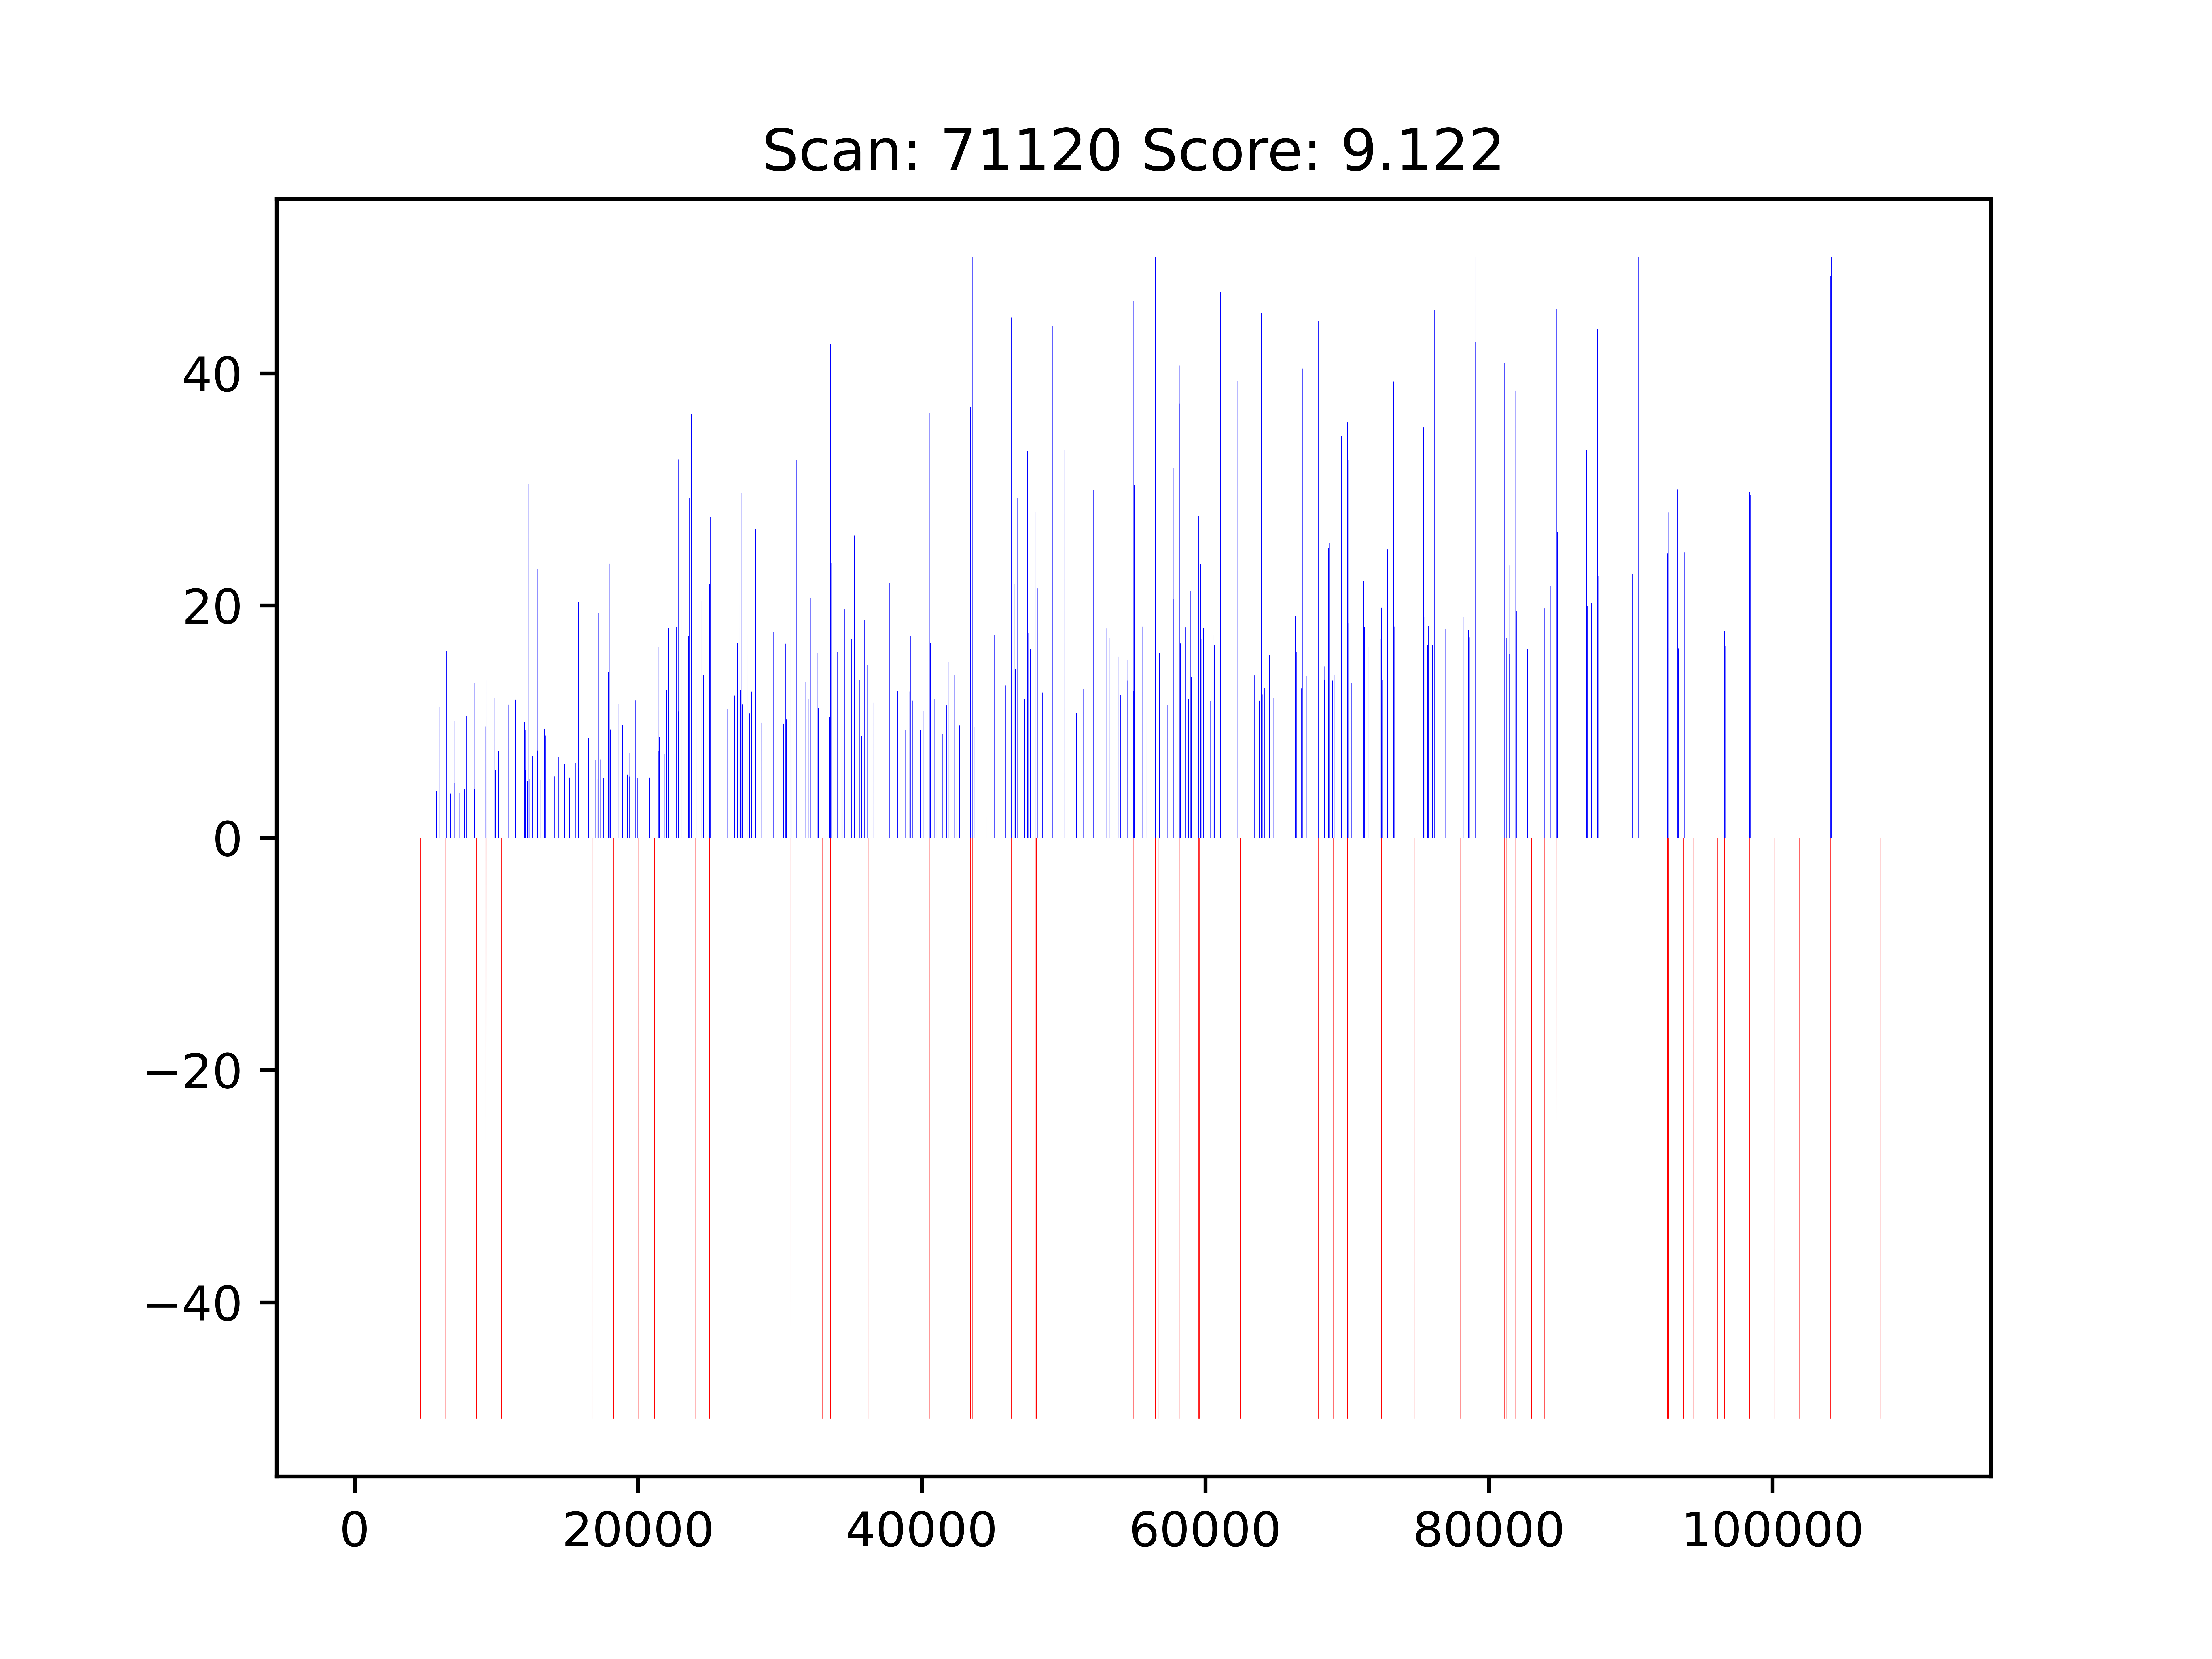
\includegraphics[width=0.95\textwidth]{figs/scan_71120_ps=False.png}
   \caption{}
   \label{fig:theo} 
\end{subfigure}
\begin{subfigure}[b]{1\textwidth}
   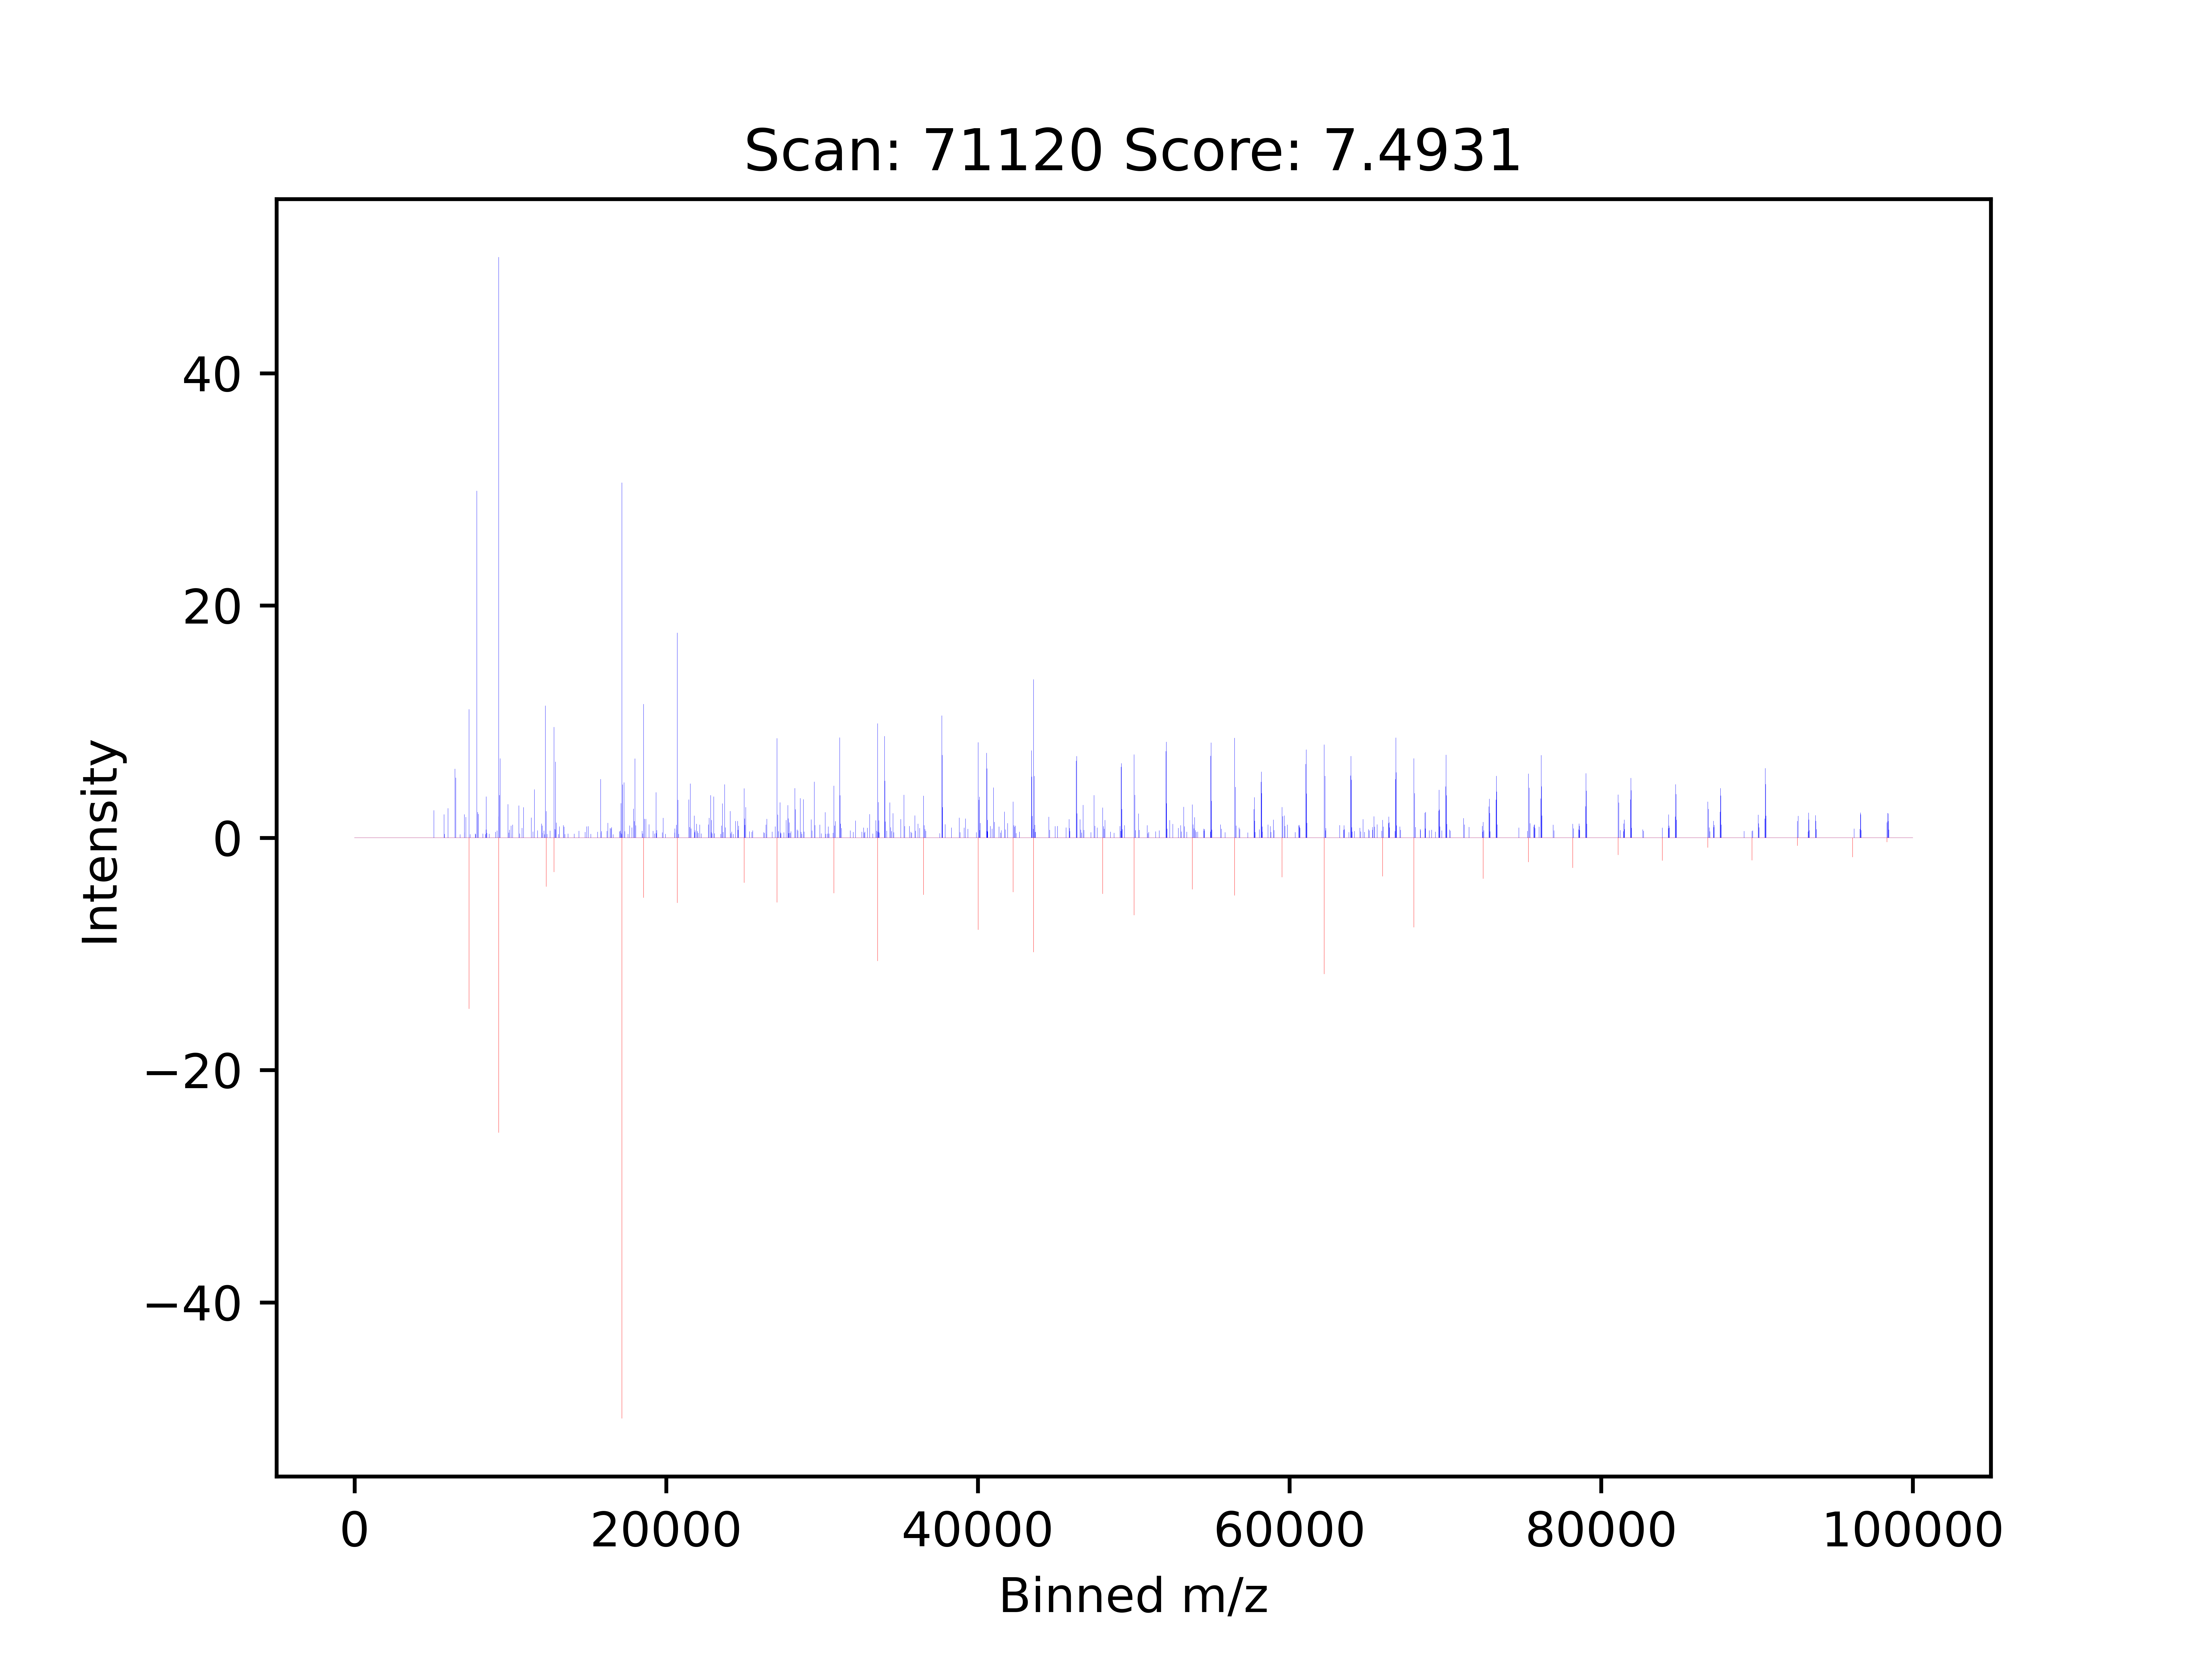
\includegraphics[width=0.95\textwidth]{figs/scan_71120_ps=True.png}
   \caption{}
   \label{fig:predict}
\end{subfigure}
\caption{(a): Plot of an experimental processed spectrum (blue) and theoretical spectrum (red). (b): experimental (blue) and predicted spectrum (red) for scan 71220 in \cref{fig:output}. Red colored spectra are presented negative only for visualization purposes.}
\label{predandtheo}
\end{figure}

\begin{figure}
\centering
\begin{subfigure}[b]{1\textwidth}
    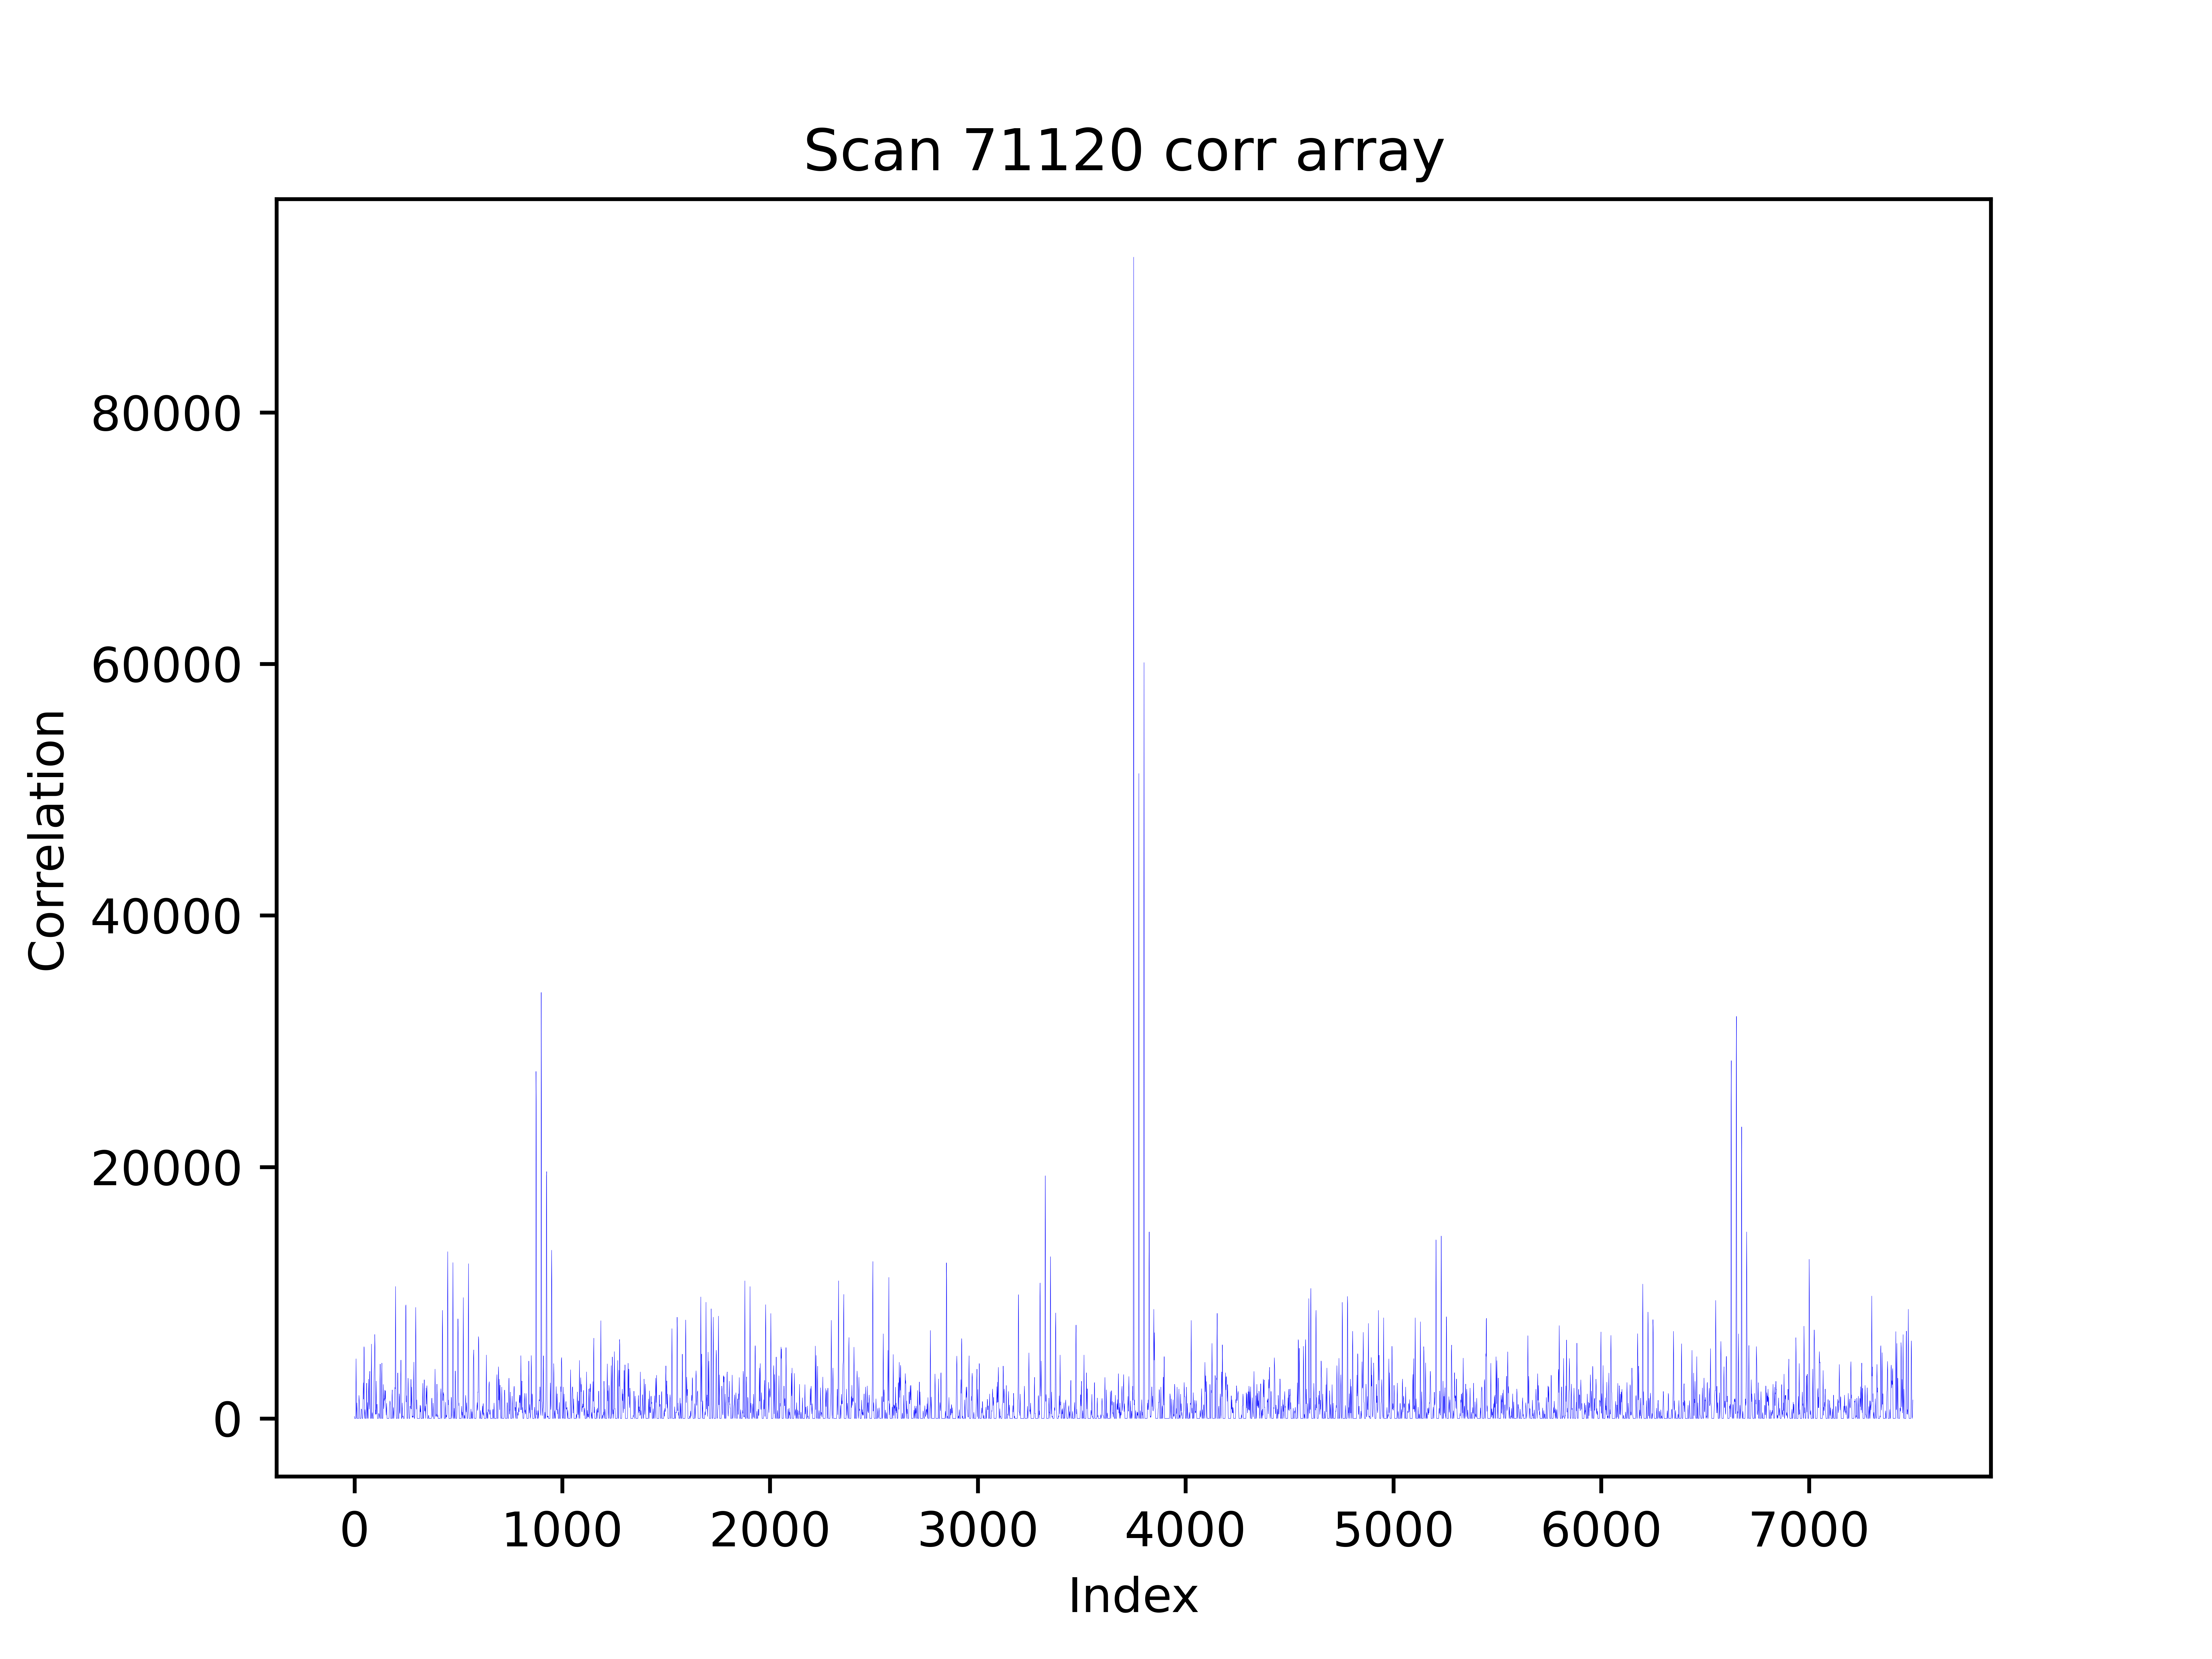
\includegraphics[width=0.95\textwidth]{figs/corrtheo.png}
   \caption{}
   \label{fig:corrtheo} 
\end{subfigure}
\begin{subfigure}[b]{1\textwidth}
   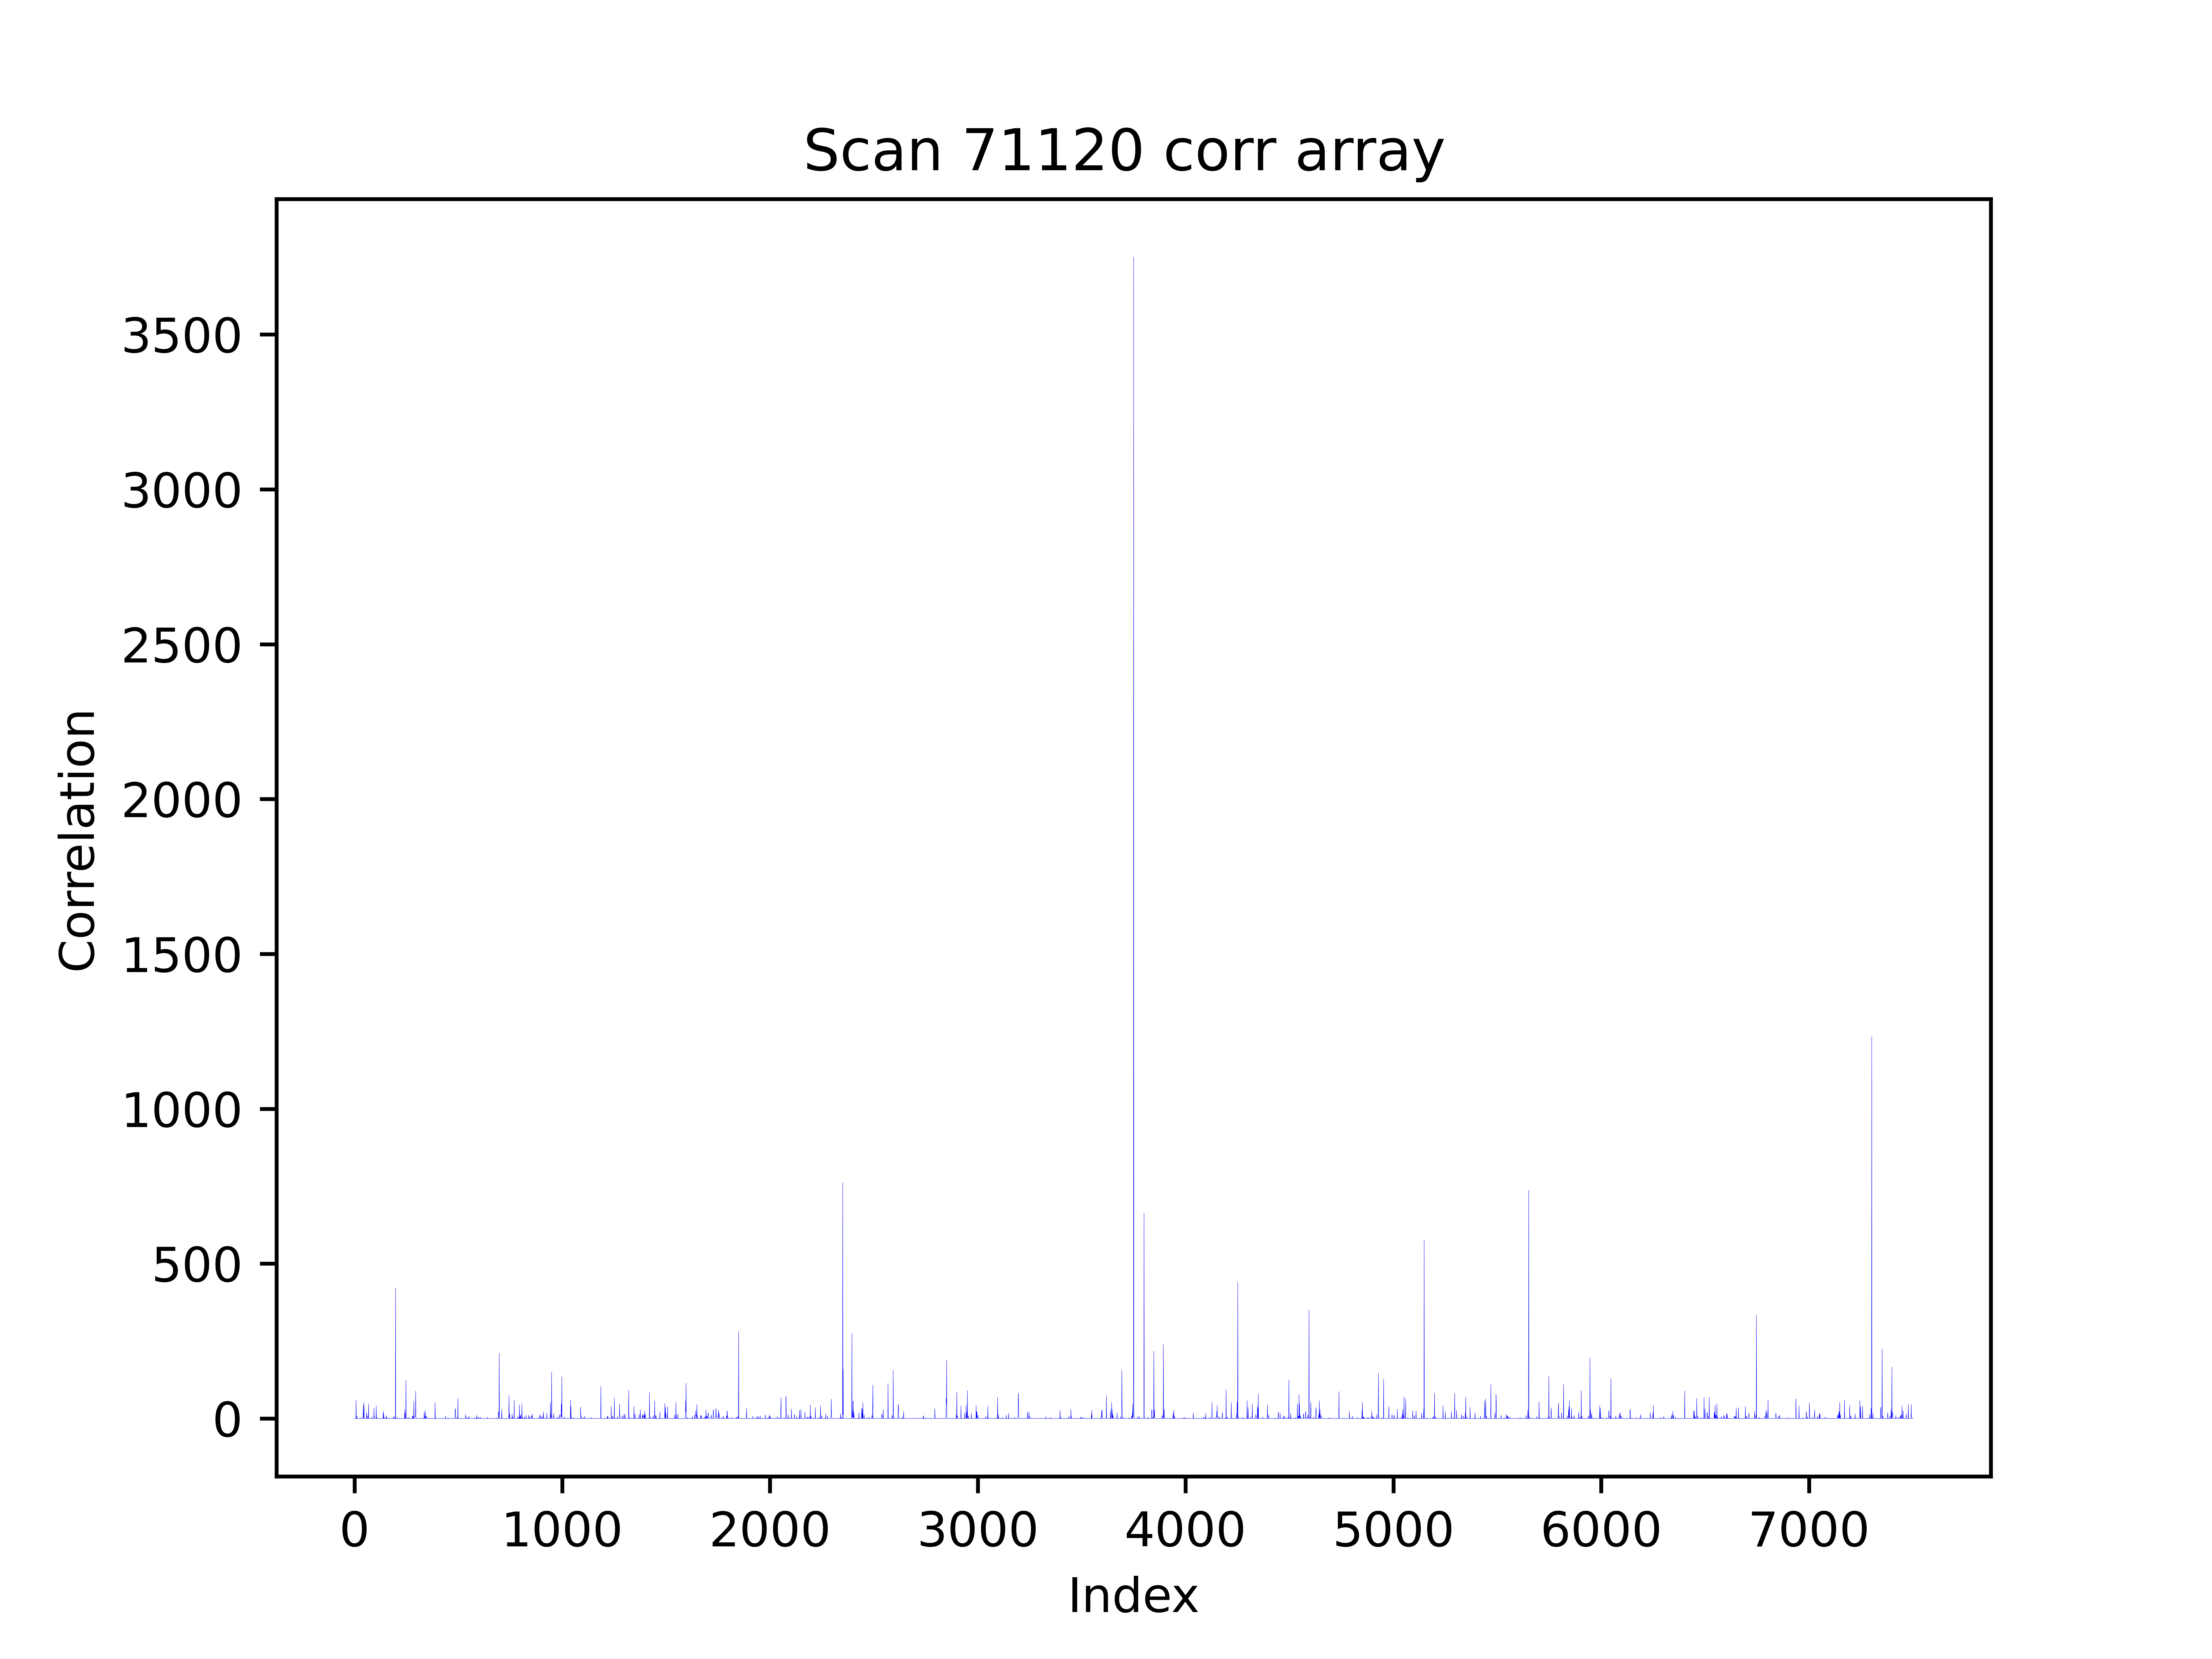
\includegraphics[width=0.95\textwidth]{figs/corrpredict.png}
   \caption{}
   \label{fig:corrpredict}
\end{subfigure}
\caption{(a): Plot of correlation array for match with theoretical spectrum (b): with predicted spectrum \cref{fig:output}}
\label{predandtheocorr}
\end{figure}

\subsubsection{Performance comparison}
Early into the development it was clear that the speed of the Python tool would be slower than the original C++ program. The main reason for this is the programming languages that were used. 

Although Python might be considered a comfortable and faster language for development by some people, it is a higher level language than C++. Python is a interpreted language, meaning that code is interpreted at run-time, while C++ is a compiled language and the code is already translated to machine language before execution. C++ programs are running directly on the hardware of the system, so there is no intermediate layer. Python programs have an interpreter as an intermediate layer, which leads to additional overhead.

C++ programs are running directly on the hardware of the system, so there is no intermediate layer. Python programs have an interpreter as an intermediate layer, which leads to additional overhead.

Memory management is different in Python and C++, C++ gives the developer more control over memory allocation than python, the performance of python on the other hand can suffer for the reason of object immutability, because it increases memory usage. 

The difference in runtime optimization is a reason for the speed difference as well: C++ code is optimized mostly at compile time, this can be e.g. loop unrolling or function inlining. Pythons standard interpreter doesn't perform optimization like this. The Type system in both programming languages is different, in C++ the variable data types are static, that means that a variable is assigned a definite data type, which can help the compiler in optimization. Python has the dynamic data type system i.e. the data type of a variable is determined at the runtime, which has a certain time cost.

The fast scoring algorithm of comet has not been implemented in this python version, which is one of the reasons for the slower performance.

At this point it needs to be noted that Python was not selected as the programming language for the sake of execution speed, but because of compatibility with the MS2PIP peptide prediction tool.

The execution times are shown in \cref{tab:speed-comparison}. 

\begin{table}[]
\begin{tabular}{|l|l|l|}
\hline
Comet Original Implementation & \begin{tabular}[c]{@{}l@{}}Python reimplementation\\ with theoretical spectra\end{tabular} & \begin{tabular}[c]{@{}l@{}}Python reimplementation\\ with predicted spectra\end{tabular} \\ \hline
0:0:37                        & 0:10:32                                                                                    & 0:17:44                                                                                  \\ \hline
\end{tabular}
\caption{Speed comparison between comet and the python reimplementation}
\label{tab:speed-comparison}
\end{table}

\subsubsection{Tests}
All functions are thoroughly tested by the Python Unittest framework.

\subsubsection{Documentation}
For description of the functions and modules in the written code, the numpy styled documentation "numpydoc" was used. Based on this, an HTML documentation with the sphinx tool is generated.

\section{Discussion and Conclusion}
In the result section of this thesis the speed and identification of the use of theoretical spectra versus the use of predicted spectra have been compared, where it became apparent that the prediction of the peptide intensity is significantly slower than the comet approach. 

\subsection{Evaluation}
\subsection{Future Work}
Comet uses multiple scores to evaluate peptide matches, e.g. the e-value of the sp\_score , so one of the key points for future work is implementing more scores with the usage of predicted spectra as well.

For the estimation of false positives comet has implemented decoy-search, this is done by reversing peptide sequences, keeping their N or C-Terminal amino acids in place, and adding these reversed peptides to the search. False positive estimation like this can lead to better identification quality.

Regarding the speed factor of this implementation, it is necessary to implement the fast scoring array manipulation like it is used in Comet to increase execution speeed.

Speed can also be greatly increased by implementing sparse arrays like they are used in comet. In this implementation, after the binning stage of either the theoretical, predicted or experimental spectra, the resulting binned arrays have a length of about 100.000, of which about 99\% values contain zeros. This is highly impractical and can significantly slow down the execution time of the program, considering that the calculation of correlation on these binned arrays has to be done hundred thousands of times in one program run.

More modifications can be considered in the future, including N and C Terminal modifications.

Since comet is highly parametrized and thus gives the user a high amount of flexibility with the program, more parameters need to be implemented in this program.

\subsection{Impact \& Conclusion}


\printbibliography

\end{document}
